%
% IAT 267: Introduction to Technological Systems
% Project Report
%
% Author: Jeffrey Leung
%

\documentclass[10pt, oneside, letterpaper, titlepage]{article}
\usepackage[utf8]{inputenc}

\usepackage[justification=centering]{caption}
    %\captionsetup[table]{skip=10pt}
\usepackage[ampersand]{easylist} % For 8-level simulations of itemize using easylist
	\ListProperties(
		Progressive*=5ex,
		Space=5pt,
		Space*=5pt,
		Style1*=\textbullet\ \ ,
		Style2*=\begin{normalfont}\begin{bfseries}\textendash\end{bfseries}\end{normalfont} \ \ ,
		Style3*=\textasteriskcentered\ \ ,
		Style4*=\textperiodcentered\ \ ,
		Style5*=\textbullet\ \ ,
		Style6*=\begin{normalfont}\begin{bfseries}\textendash\end{bfseries}\end{normalfont}\ \ ,
		Style7*=\textasteriskcentered\ \ ,
		Style8*=\textperiodcentered\ \ ,
		Hide1=1,
		Hide2=2,
		Hide3=3,
		Hide4=4,
		Hide5=5,
		Hide6=6,
		Hide7=7,
		Hide8=8 )
%\usepackage{geometry}
	%\geometry{margin=1.2in}
\usepackage{graphicx}
	\graphicspath{ {img/} }
\usepackage[colorlinks=true, linkcolor=blue]{hyperref}
\usepackage[final]{pdfpages}  % Allows inclusion of PDFs
\usepackage{verbatim}

\renewcommand{\arraystretch}{1.2}
\renewcommand{\baselinestretch}{1.5}

% Font-related commands:
\usepackage[T1]{fontenc}  % Allows the use of symbols in LMSS such as the braces
\usepackage[default, osfigures]{opensans}
\usepackage{textcomp} % Allows the use of symbols in LMSS such as textasterisk and textbullet
\renewcommand{\familydefault}{\sfdefault}

\begin{document}

	\begin{titlepage}
		\begin{center}

			\vspace{15cm}
			\textsc{\Large IAT 267: Introduction to Technological Design}\\
			\vspace{1cm}
			\textsc{\Large Spring 2016, Section D100/101} \\
			\vspace{3.5cm}
			\textsc{\Large Project Report: Batman Item Reminder Device} \\
			\vspace{2cm}

			\begin{tabular}[c]{ l }
				Leung, Jeffrey \\
				Li, Zheyang  \\
				Li, Mina \\
				Pinto, Paul
			\end{tabular}
			\vspace{5cm}

		\end{center}
	\end{titlepage}

	\tableofcontents
	\clearpage

	\section{Project Overview}

		The \emph{Batman Item Reminder Device} (which shall henceforth be referred to as \emph{BIRD}) is a passively monitoring, smart home, Processing and dual-Arduino technological system created to ensure that the user has their required items for the day. The presence of items are monitored and notification consisting of LEDs and a sound will alert the user if they do not have all of their items with them. The purpose of the system is to take the human factor out of remembering items and only remind the user when absolutely necessary (i.e. only when an item has been forgotten).

		BIRD consists of three interactive systems:

		\begin{enumerate}

			\item The car box system (henceforth referred to as \emph{C-Box}), which alerts the user if they have left any items on the pressure pads,
			\item The item detection system with pressure pads (henceforth referred to as \emph{P-Pad}), which sends the presence of any item on the pressure pads to the C-Box, and
			\item The Processing application which shows the status of the pressure pads (i.e. activated vs. not activated) and allows the user to delay activation of the pressure pad system to a specified date and/or time.

		\end{enumerate}

		\subsection{Ideation}

			Our idea process began with us discussing widely varying possibilities in order to find a viable, fun, and useful concept to implement. Any and all ideas were considered in our attempt to find the best project to work with.

			\begin{quote}
				``I'll be honest - we're throwing science at the wall here to see what sticks. No idea what it'll do. Probably nothing. Best-case scenario, you might get some superpowers. Worst case, some tumors, which we'll cut out.''
				\hfill -- Cave Johnson, \emph{Portal 2}
			\end{quote}

			An example of an idea we considered was a physical-to-digital whiteboard, which had already been developed by a team (\href{https://www.reddit.com/r/arduino/comments/2w4s1y/digitally_encoding_a_chalkboard_with_arduino/}{Reddit discussion}, \href{https://www.youtube.com/watch?v=y1aw0IiamFM}{video demonstration}, \href{https://github.com/string2string/string2string}{source code on GitHub}). This project would allow instant digitalization of diagrams and equations written on a chalkboard or whiteboard, so teachers could easily send written material to students. However, there was little area to expand upon the idea, but consideration of this idea helped us to realize we wanted something that would be useful to someone in some way, rather than an art piece, and it also improved out ability to be able to analyze a project and suggest improvements.

			Another idea we considered was a calendar consisting of a grid of LEDs, which represents whether or not a user has an event on any given day. This would greatly simplify project organization and scheduling, as well as sync seamlessly with Google Calendar for easy usage. A similar idea utilizing Lego bricks was designed by a studio named Vitamins, and can be found \href{http://www.bit-planner.com/}{here}. Unfortunately, this was not as universal as we would prefer as it might only appeal to a niche audience. Exploring this idea further set in stone our desire to create a primarily useful system rather than a primarily creative device, and it reminded us of the target scope of the project.

		\subsection{Research}

			After choosing our idea, we researched industry and indie implementations of similar ideas.

			One such concept was the \href{https://www.thetileapp.com/}{Tile}, a tag which attaches to items and can be buzzed from a phone or vice versa. Tile, however, requires a battery which is not replaceable by the user and clutters up your keychain further. We wanted our system to use replaceable batteries or external power, and to not clutter up your everyday items.

			Another concept we studied was the \href{https://www.kickstarter.com/projects/416260479/smartwallit-pro-new-smartwallit-new-experience/description}{SmartWallit}, a card inserted into a wallet and connected wirelessly to a phone. This device, funded on Kickstarter, alerts users when their wallet and phone are far apart from each other, and can play a sound on either the wallet or the phone if one is lost. This shared our idea of monitoring items passively for the user. However, SmartWallit only works between a phone and a wallet, which must be in close proximity; we wanted our system to be more versatile and configurable in multiple ways by the user.

		\subsection{Interaction Model}

			To use the system, the user selects items they want to reminded of and places them on the P-Pad. If they would like to deactivate the P-Pad for an indefinite amount of time, the user should touch the P-Pad capacitive sensor to turn the system off (and touch it again to turn the system on). A labeled LED indicates whether the system is currently activated or deactivated.

			When the user gets into their car, if the P-Pad is activated and the user has left their items on the P-Pad, then the C-Box will play an alert sound and blink LEDs to indicate that there are items left on the P-Pad. To deactivate the alarm, the user simply get out of the car, or press the power button on the C-Box to deactive the C-Box for several minutes.

			The Processing application augments the P-Pad with greater flexiblity and customization, and allows the user to choose the next time to activate the P-Pad. For example, the user can leave a specific item on the P-Pad, set the delay for 3 days, and not have the C-Box alert them of the item until 3 days from now.

	\clearpage
	\section{Physical Structure}

		\subsection{Pictures and Schematics}

			Figure~\ref{fig:sketch} shows the initial concept for the physical systems.

			\begin{figure}[!htb]
				\centering
				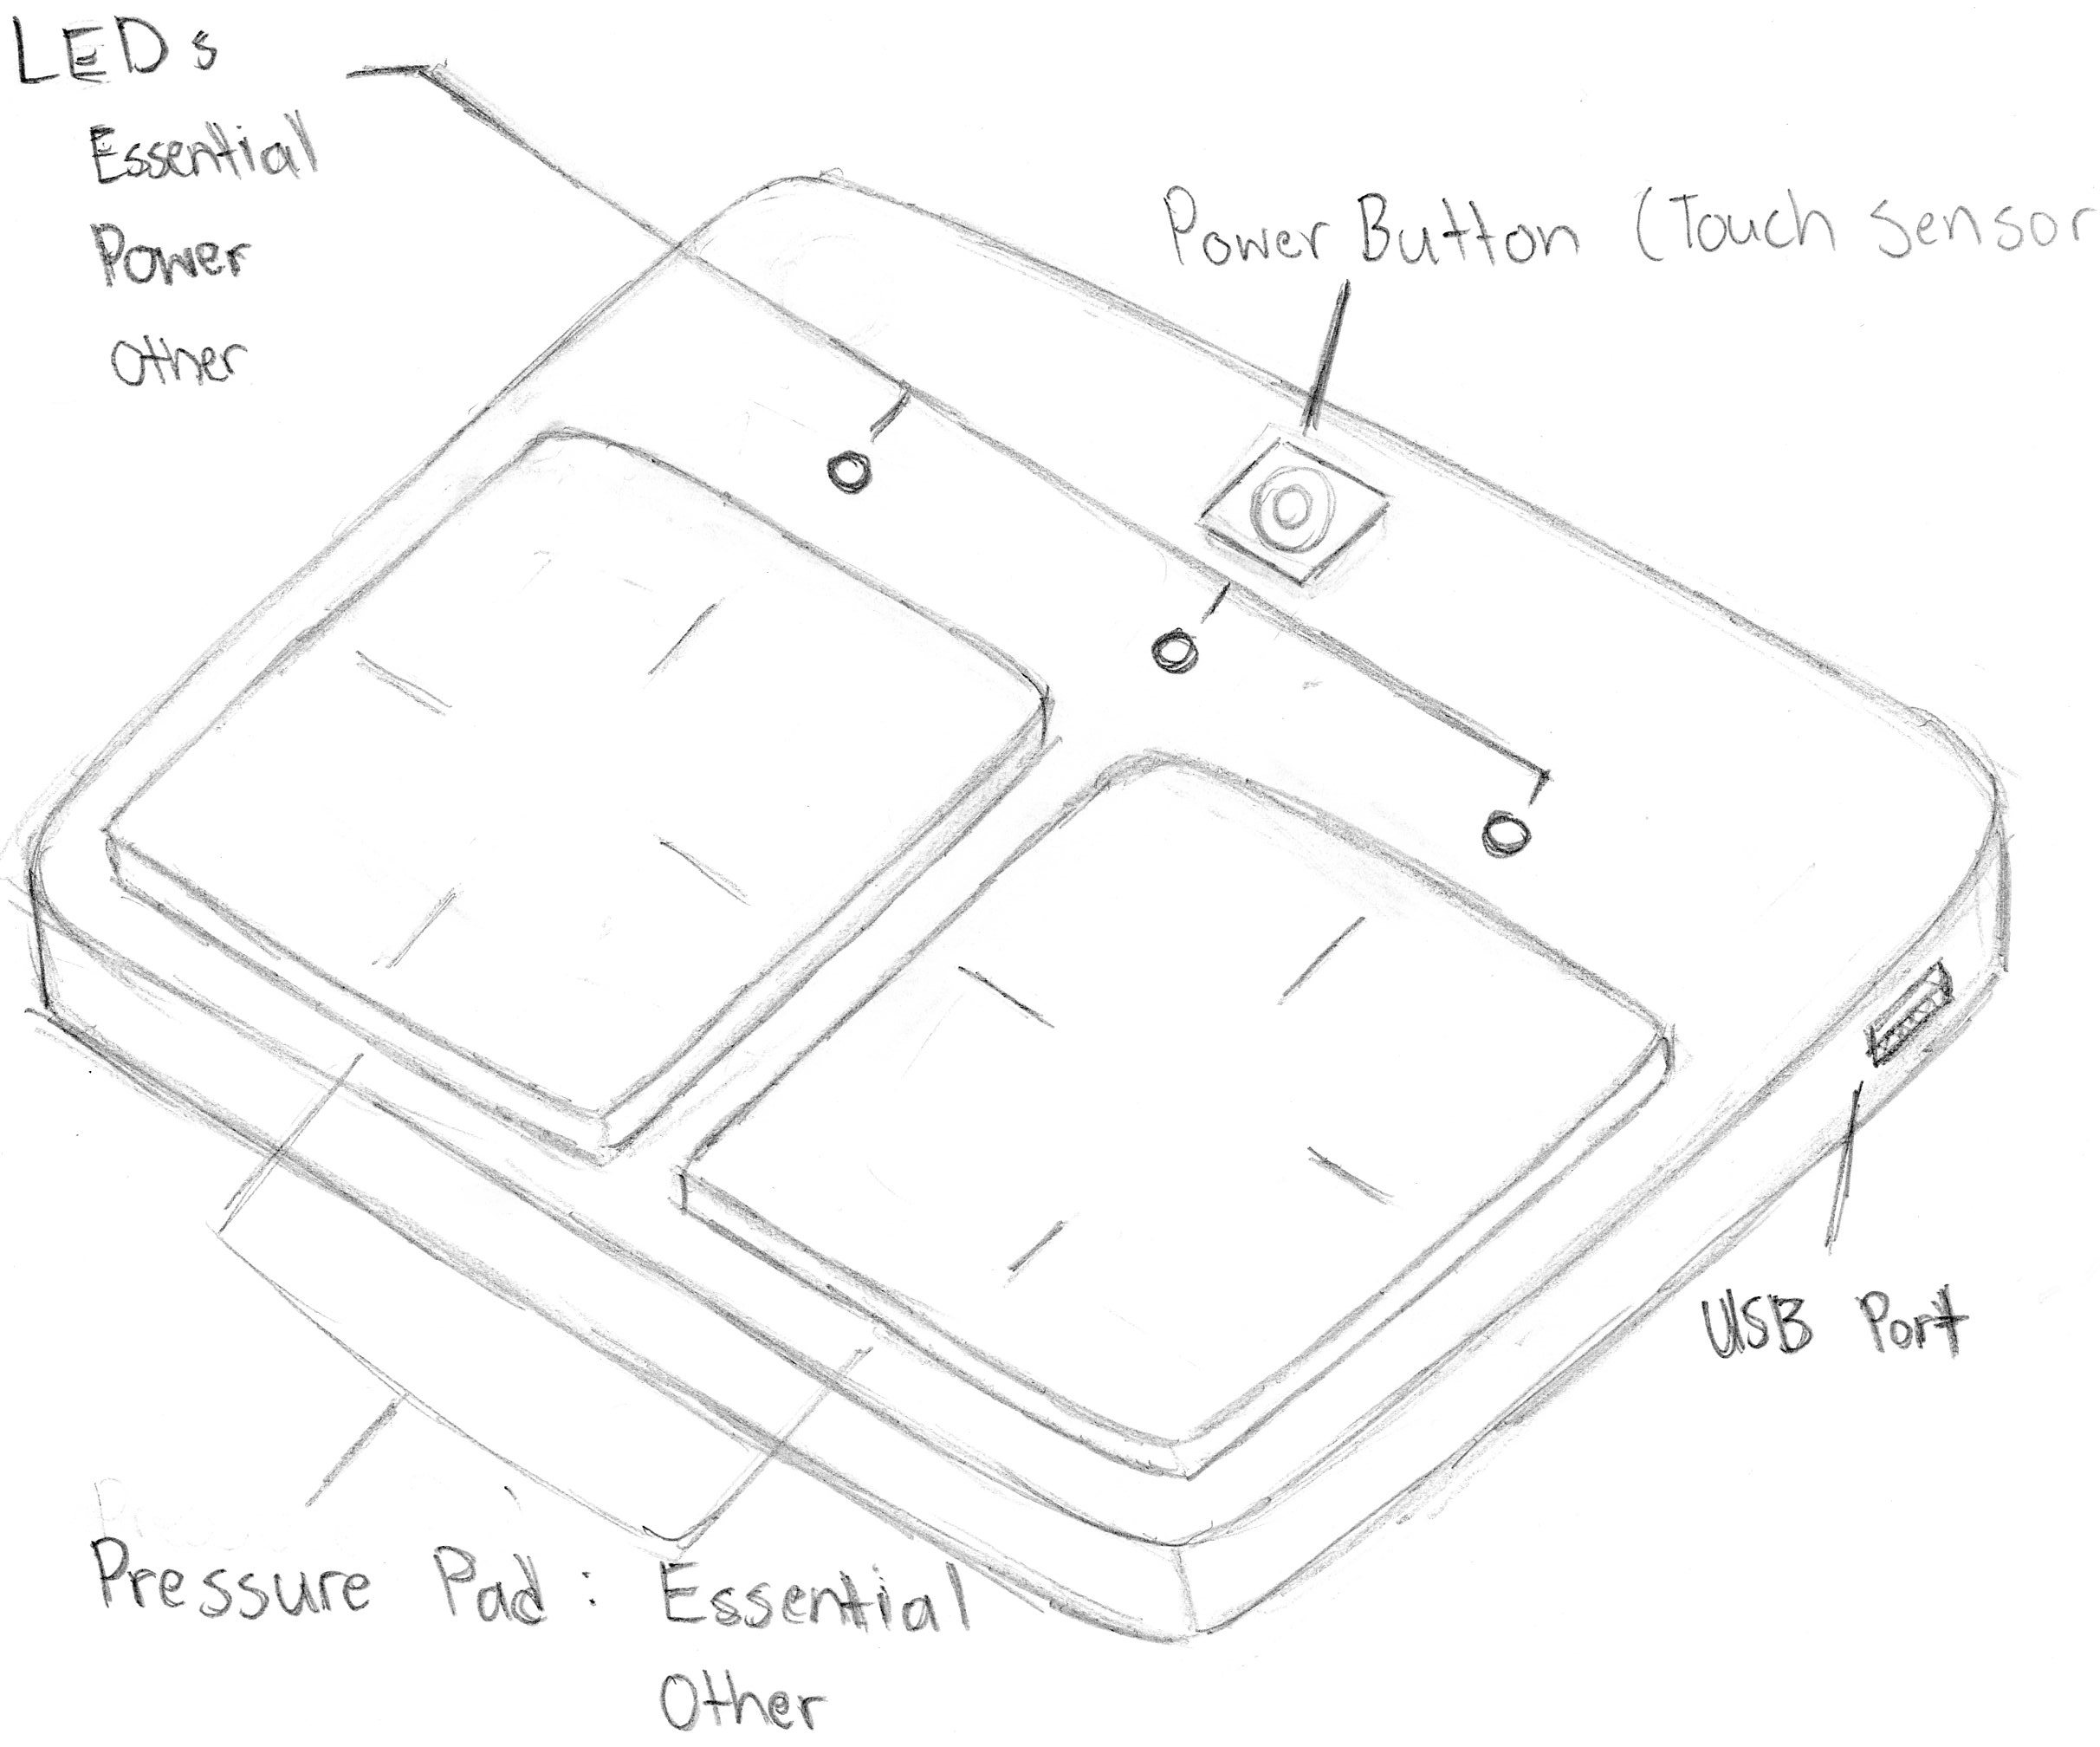
\includegraphics[width=25em]{sketch-p-pad}
				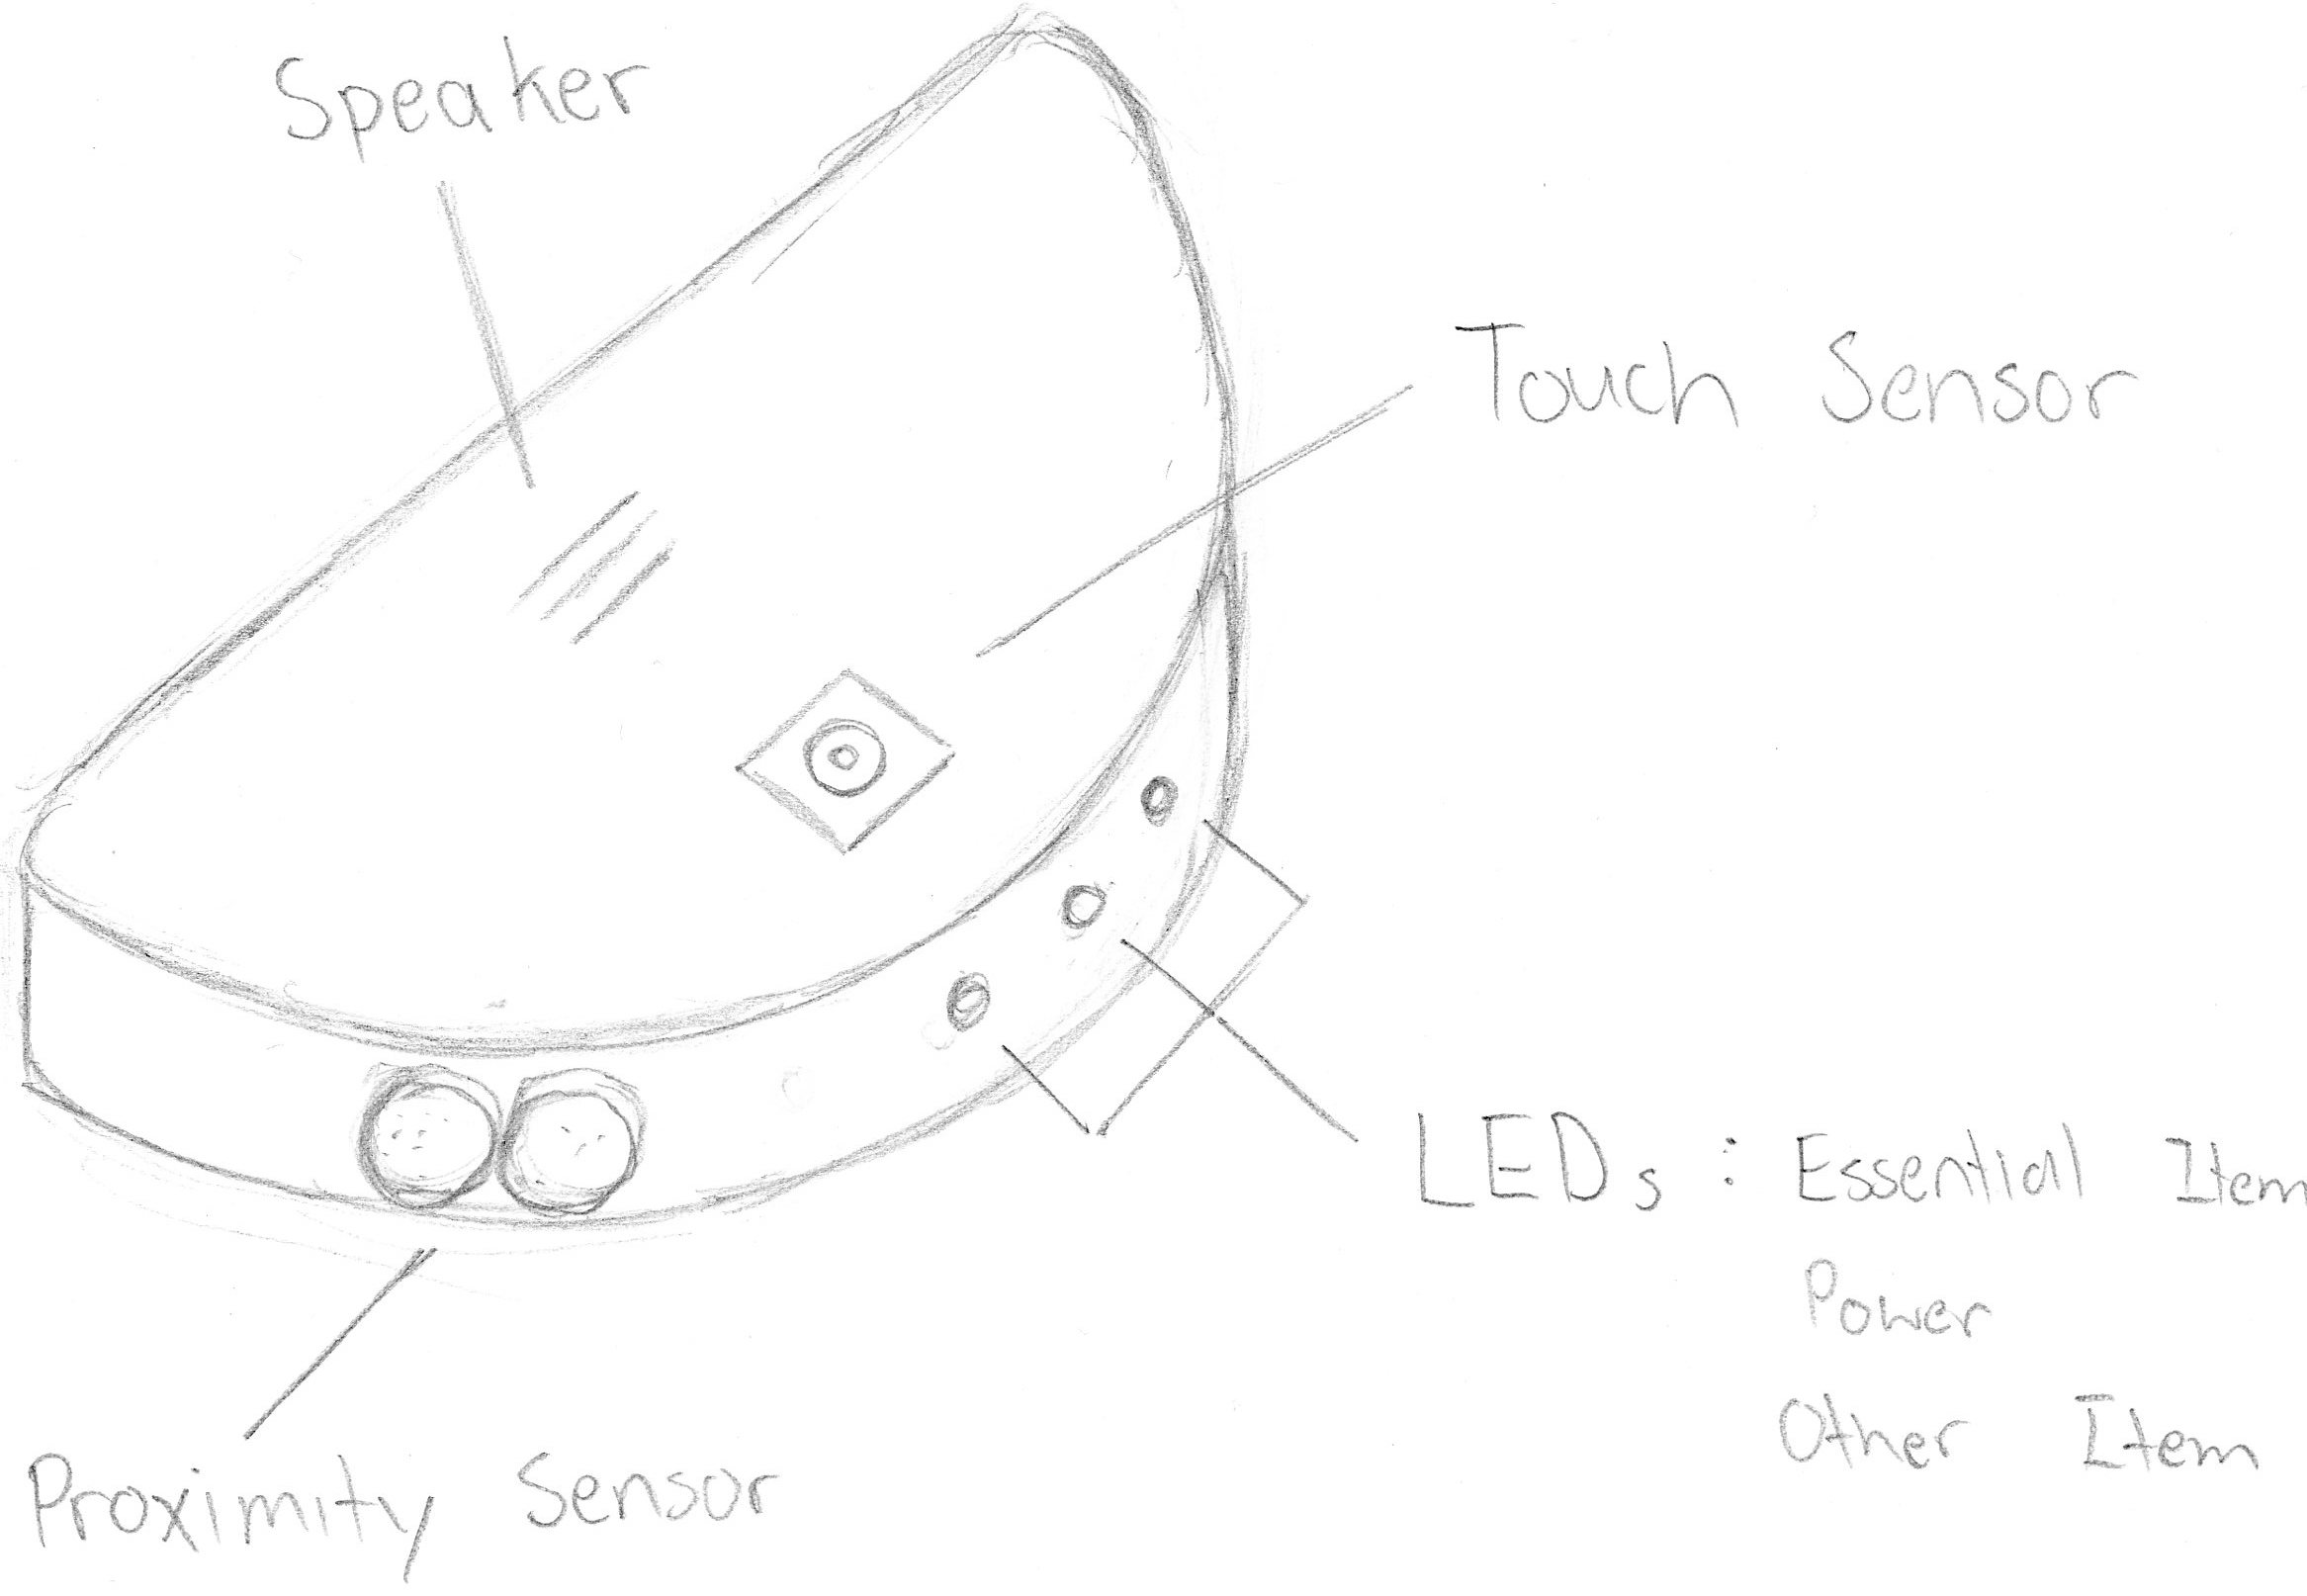
\includegraphics[width=25em]{sketch-c-box}
				\caption{Concept for the Physical Systems}
				\label{fig:sketch}
			\end{figure}

			\clearpage
			Figure~\ref{fig:picture-m2} shows the prototypes as presented for Milestone 2.

			\begin{figure}[!htb]
				\centering
				\includegraphics[width=25em]{img/picture-m2-c-box}
				\includegraphics[width=25em]{picture-m2-p-pad}
				\caption{Prototype at Milestone 2 (Top: C-Box, bottom: P-Pad)}
				\label{fig:picture-m2}
			\end{figure}

			\clearpage
			Figure~\ref{fig:picture-m3} shows the final product as presented for Milestone 3.

			\begin{figure}[!htb]
				\centering
				\includegraphics[width=25em]{picture-m3}
				\caption{Final Product at Milestone 3 (Top: C-Box, bottom: P-Pad)}
				\label{fig:picture-m3}
			\end{figure}

			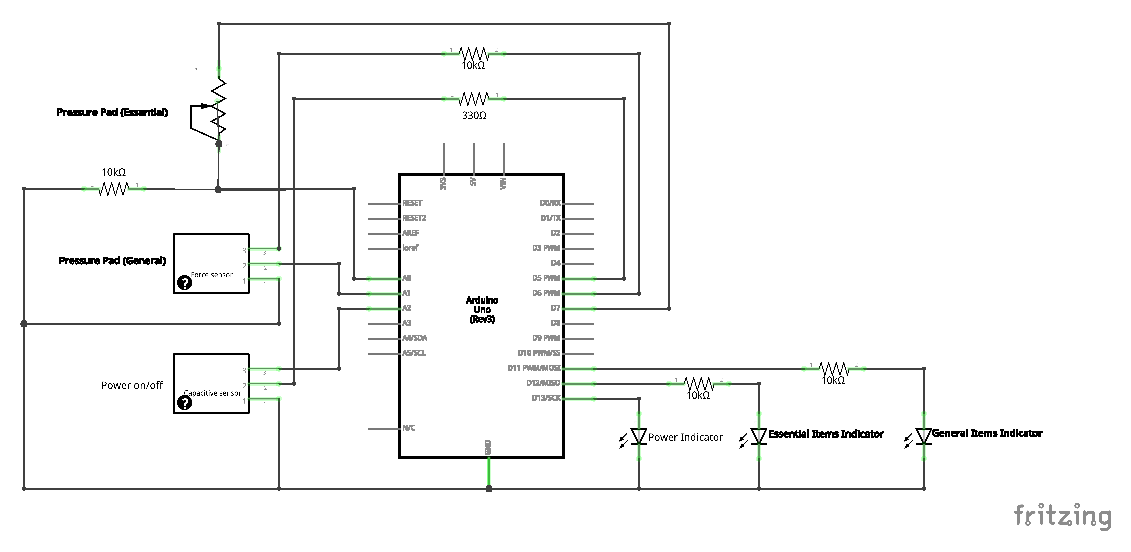
\includepdf[pages={1, 2}, scale=0.7, nup=1x2]{pdf/schematic-combined.pdf}

		\subsection{Processing Application}

			Figure~\ref{fig:processing-application} shows the interface of the Processing application.

			\begin{figure}[!htb]
				\centering
				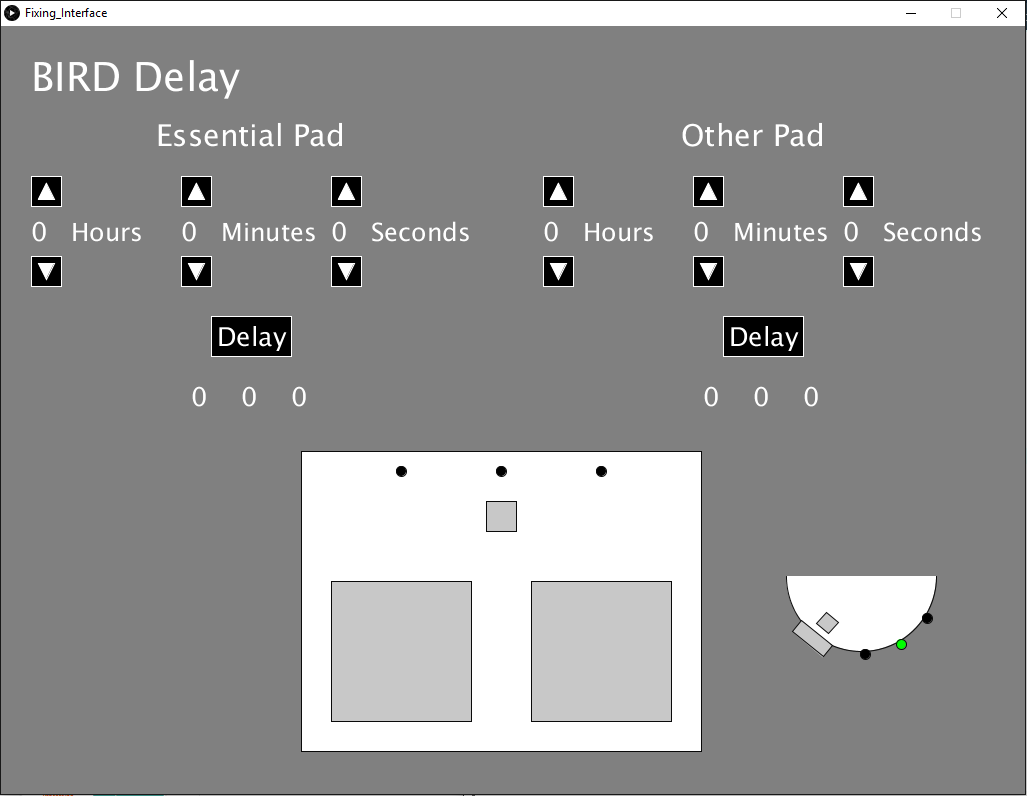
\includegraphics[width=30em]{processing-application}
				\caption{Processing Application}
				\label{fig:processing-application}
			\end{figure}

		\subsection{Code}
			The code is hosted on \href{https://github.com/jleung51/BIRD}{GitHub}.

		\subsection{Components}
			% Role of each component

			List of C-Box components:

			\begin{itemize}
				\item Arduino (1)
				\item Capacitive sensor (1) (Deactivates the system for a period of time)
				\item Ultrasonic sensor (1) (Detects the presence of the user)
				\item LED (3) (Alerts the user to the statuses of power/pressure pads)
				\item Speaker (1)
				\item Transistor (1) (Increases the power to the speaker)
			\end{itemize}

			\noindent
			List of P-Pad components:

			\begin{itemize}
				\item Arduino (1)
				\item Capacitive sensor (1) (Activates or deactivates the system)
				\item Pressure sensor (2) (Detects the presence of items on the pad)
				\item LED (3) (Alerts the user to the statuses of power/pressure pads)
			\end{itemize}

	\clearpage
	\section{Looking Back (Challenges)}

		As in any project involving collaboration, we encountered a number of issues while working on our project. Some issues related to our abilities to work together as a team, while others focused mainly on technological difficulties within the scope of our project.

		One example of an obstacle in team communication was deciding upon a single idea. While we all had numerous ideas for the project, we had a difficult time reconciling different goals and streams to settle on a common idea. Given a short deadline and multiple ideas, we sat down together to choose a concept which was viable within the scope and time of the semester, met all the requirements, and would be enjoyable to create - and we ended with a single idea.

		The greatest technological challenge we faced was how to implement wireless communication between the P-Pad and the C-Box. Our first attempt utilized Arduino Bluetooths; however, we had multiple issues in connecting them with our computers, as well as connecting the Bluetooth devices with each other. Another option we worked with was the \href{https://arduino-info.wikispaces.com/Nrf24L01-2.4GHz-HowTo}{nRF24L01+ radio frequency transmitter}. However, the required voltage proved to be too finicky to output, so this was not a viable way to communicate in our project. In the end, our final implementation did not have wireless communication due to the numerous aforementioned difficulties, as well as the inability to buy a standard, reliable set of communication modules such as xBees.

		Finally, a problem we encountered in designing the system was how to synchronize communication between the 3 concurrent systems - the Processing application, the P-Pad, and the C-Box. We iterated through numerous possibilities such as sending a delay to the Arduino from the Processing application or sending no data from the P-Pad to the Processing application, but we were able to construct a clear and functional system of communication for our final implementation by careful implementation, pair debugging, and a significant amount of testing. Our communication involves:
		\begin{enumerate}
			\item The Processing application sending whether or not the system is currently delayed to the P-Pad,
			\item The P-Pad sending the status of the pads to the Processing application to be displayed in real-time, and
			\item The P-Pad sending whether or not to activate the alerts to the C-Box, which is conditional relative to the status of the delay (received from the Processing application).
		\end{enumerate}

	\clearpage
	\section{Looking Ahead}

		Given unrestricted funds, tools, and time, there are numerous improvements we could have made to the project, such as better components or easier usage of the Processing program to control the Arduino system.

		Our final iteration used cardboard boxes altered to fit the circuitry and components. In the best-case scenario, custom-sized metal casings would be used for each system to improve the aesthetics of the project.

		The Processing program currently does not save information between sessions due to the nature of Processing; given more time, we could find a way to save the delay times in a text file, retrieve them upon startup, and alter the information as needed.

		The pressure pads currently can only detect whether or not items are present, and not how many items are on the pad or how much the items weigh. With a greater budget, we would be able to utilize more pressure pads as well as more sensitive pressure pads, so that a pad could report its status based on weight (e.g. keys taken but wallet left on the pad).

		Given a greater budget, many other components used in our project could be upgraded. For example, the infrared sensor originally used for the project was faulty and did not always react to a change in distance. The capacitive sensors used for the project would sporadically stay at a value of zero for several seconds after being touched, requiring a significant amount of patience. The speaker used to sound an alert was salvaged from computer speakers, and could be of significantly greater quality. The communication between Arduinos could be wireless and more reliable by using modules such as the more expensive xBees. The cases for the systems could be made more compact through a replacement for the Arduino such as an \href{https://www.arduino.cc/en/Main/ArduinoBoardLilyPad}{Arduino LilyPad} or an \href{https://www.arduino.cc/en/Main/ArduinoBoardProMini}{Arduino Pro Mini}.

		With our limitations in mind, our project met and exceeded our expectations, and we are proud to have created this technological system to enhance the abilities of smart-home technology.

\end{document}
